\documentclass{article}

% Language setting
\usepackage[french]{babel}

% Set page size and margins
\usepackage[letterpaper,top=2cm,bottom=2cm,left=3cm,right=3cm,marginparwidth=1.75cm]{geometry}

% Useful packages
\usepackage{amsmath}
\usepackage{graphicx}
% \usepackage[colorlinks=true, allcolors=blue]{hyperref}
\usepackage[utf8]{inputenc}
\usepackage[T1]{fontenc}
\usepackage[version=4]{mhchem}
\usepackage{siunitx}
\usepackage{enumitem}
\usepackage{pgffor}
\usepackage{ifthen}
\usepackage{caption}
\usepackage{float}     % For using [H] specifier in figure environments

\setlist{}

\title{Rappels de cours - Physique-Chimie 4ème}

\begin{document}

\sloppy  % This will apply the sloppy setting to the entire document.
\maketitle

\def\WITH_CORRECTION{NO}

\newcommand{\question}[3]{%
    \noindent\textbf{#1} \\[0.5em] % Print the question in bold, with some spacing after
    \ifthenelse{\equal{\WITH_CORRECTION}{NO}}{%
        % If \WITH_CORRECTION is NO, print lines for answers
        \foreach \i in {1,...,#2} {%
            \noindent\makebox[\linewidth]{\dotfill}%
            \ifnum\i<#2\\[0.5em] \fi % Add spacing after the line except for the last one
        }
    }{%
        % If \WITH_CORRECTION is YES, print the answer
        \noindent\parbox{\linewidth}{#3}
    }%
}

\newcommand{\character}[1]{%
    \foreach \i in {1,...,#1} {%
        .%
    }%
}

\newcommand{\trou}[2]{%
    \ifthenelse{\equal{\WITH_CORRECTION}{NO}}{%
        \noindent\character{#1}
    }{%
        \noindent#2 % Print the answer
    }%
}

\section{Organisation et transformation de la matière}

\subsection{Les atomes et les molécules}

\begin{enumerate}[itemsep=0pt]
  \item \question{Quelle est la différence entre un atome et une molécule ?}{2}{Une molécule est constituée d'atomes}
  \item \question{Quelle est la formule brute de la molécule d'eau ?}{1}{\ce{H2O}}
  \item \textbf{Tests d'identification}
  \begin{itemize}
      \item[$\bullet$] \question{Quel test permet d'identifier la présence d'eau (\ce{H2O}) dans un mélange ?}{1}{Test de la glace ou du bleu de cobalt}
      \item[$\bullet$] \question{Quel test permet d'identifier la présence de dioxyde de carbone (\ce{CO2}) dans un mélange ?}{1}{Test à la chaux éteinte}
      \item[$\bullet$] \question{Quel test permet d'identifier la présence de dioxygène (\ce{O2}) dans un mélange ?}{1}{Test de la flambée}
      \item[$\bullet$]  \question{Quel test permet d'identifier la présence de dihydrogène (\ce{H2}) dans un mélange ?}{1}{Test de la détonation}
  \end{itemize}
  \item \question{Quels sont les 3 états de l'eau ?}{1}{Solide, liquide, gazeux}
\end{enumerate}

\subsection{La masse volumique}


\begin{enumerate}
    \item \question{Quelle est la formule de la masse volumique ?}{1}{\(\rho = \frac{m}{V}\)}
    \item \question{Quelle est la masse volumique de l'eau ?}{1}{\(\SI{1000}{\kilogram\per\cubic\meter}\)}
    \item \textbf{Conversion des unités :}
    \begin{itemize}
        \item[$\bullet$] 1 kg = \trou{8}{1000} g
        \item[$\bullet$] \num{1} \unit{\cubic\meter} = \trou{8}{1000} L
        \item[$\bullet$] 1 L = \trou{8}{1000} \unit{\cubic\cm}
        \item[$\bullet$] 1 \unit{\mL} = \trou{8}{1} \unit{\cubic\cm}
    \end{itemize}
    \item \question{Comment détermine-t-on qu'un solide flotte sur ou coule dans l'eau ?}{1}{Un solide flotte s'il est moins dense que l'eau et coule s'il est plus dense.}
\end{enumerate}

\subsection{La structure de l'Univers et du système solaire}
\begin{enumerate}
    \item \question{Quelle est la définition d'une unité astronomique ? Et d'une année lumière ? Ce sont des durées, des vitesses ? Des distances ?}{2}{Une unité astronomique (UA) est la distance moyenne entre la Terre et le Soleil, et une année-lumière (al) est la distance parcourue par la lumière en un an. Ce sont des distances.}
    \item \question{Si on connaît la vitesse de la lumière, comment peut-on retrouver la valeur d'une année lumière ?}{2}{En multipliant la vitesse de la lumière par le nombre de secondes dans une année.}
    \item \question{Pourquoi dit-on qu'on voit les astres tels qu'ils étaient dans le passé ? Pour information, la proxima du Centaure est à une distance de 4.22 a.l.}{2}{Parce que la lumière met du temps à voyager jusqu'à nous. Nous voyons les objets tels qu'ils étaient au moment où la lumière a quitté ces objets.}
\end{enumerate}

\section{Mouvement et intéractions}
\subsection{La vitesse d'un système en mouvement}
\begin{enumerate}
    \item \question{Quelle est l'expression de la vitesse en fonction du temps et de la distance ?}{2}{\( v = \frac{d}{t} \)}
\end{enumerate}

\subsection{Le poids}
\begin{enumerate}
    \item \question{Quelle est la différence entre le poids et la masse ? Quelles sont leurs unités respectives ? Quelle est l'unité de l'intensité de pesanteur ? Bonus : quelle est la valeur de l'intensité de pesanteur ?}{4}{La masse est la quantité de matière et se mesure en kilogrammes (kg). Le poids est la force exercée par la gravité sur un objet et se mesure en newtons (N). L'unité de l'intensité de pesanteur est le mètre par seconde au carré (\(\text{m/s}^2\)). La valeur standard de l'intensité de pesanteur est environ \(9.81 \text{ m/s}^2\).}
    \item \question{Quelle est la différence entre le poids et la masse ? Quelles sont leurs unités respectives ?}{2}{La masse est une mesure de la quantité de matière (kg) et le poids est la force due à la gravité (N).}
\end{enumerate}

\section{L’énergie et ses conversions}
\subsection{Les lois de la tension et de l'intensité électriques}
\begin{enumerate}
    \item \question{Quelle est l'unité de l'intensité électrique ? Quel instrument permet de mesurer l'intensité électrique ?}{1}{L'unité de l'intensité électrique est l'ampère (A). L'instrument utilisé est l'ampèremètre.}
    \item \question{Comment le branche-t-on dans un circuit (pour mesurer l'intensité électrique) ?}{3}{Il se branche en série avec le circuit.}
    \item \question{Quelle est l'unité de la tension électrique ? Quel instrument permet de mesurer l'intensité électrique ?}{1}{L'unité de la tension électrique est le volt (V). L'instrument utilisé est le voltmètre.}
    \item \question{Comment le branche-t-on dans un circuit (pour mesurer la tension électrique) ?}{3}{Il se branche en parallèle avec le circuit.}
    \item \question{Dans le circuit ci-dessous, quelle est la valeur de l'intensité dans le circuit ? Quelle loi permet de déterminer cette valeur ?}
    {1}
    {\(I_1 = I_2 = I_3\). Loi d'unicité de l'intensité électrique : L'intensité électrique est la même dans un circuit en série ou dans une branche d'un circuit en dérivation. \\ 
    L'intensité est la même en tout point d'une même branche d'un circuit électrique}
    \begin{figure}[H]
        \centering
        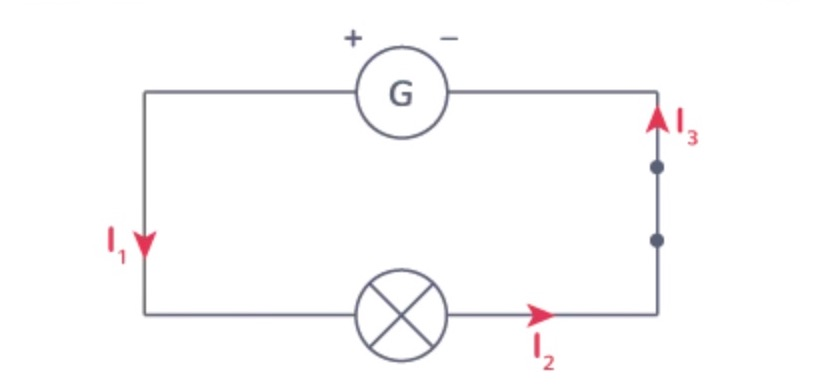
\includegraphics[width=0.5\linewidth]{intensite_circuit_1.jpg}
        \caption{\label{fig:intensite_circuit_1} Circuit électrique 1}
    \end{figure}
    \item \question{Dans le circuit ci-dessous, quelle est la valeur de l'intensité du générateur ? Quelle loi permet de déterminer cette valeur ?
    \begin{minipage}{\textwidth}
        \centering
        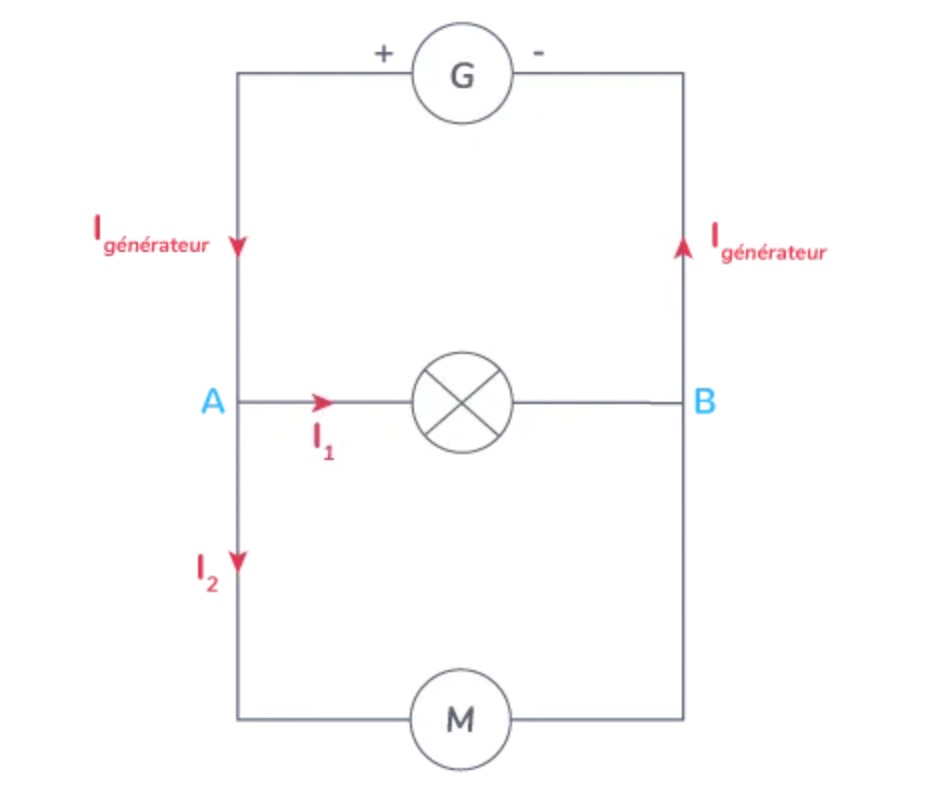
\includegraphics[width=0.5\linewidth]{intensite_circuit_2.jpg}
        \captionof{figure}{Circuit électrique 2}
    \end{minipage}}{1}{\(I_\text{générateur} = I_1 + I_2\). Loi d'additivité de l'intensité électrique. Dans un circuit en dérivation, la somme des intensités qui arrivent sur un noeud est égale à la somme des intensités qui en repartent}
    \item \question{Dans le circuit ci-dessous, quelle est la relation entre \(U_\text{générateur}\), \(U_L\), et \(U_M\) ? Quelle loi permet de déterminer cette valeur ? \\
    \begin{minipage}{\textwidth}
        \centering
        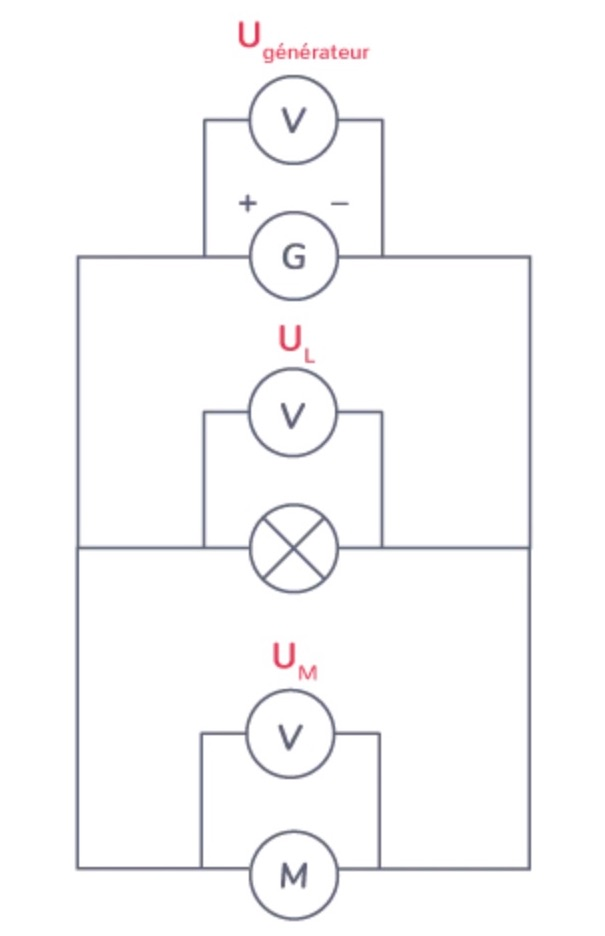
\includegraphics[width=0.5\linewidth]{tension_circuit_1.jpg}
        \captionof{figure}{Circuit électrique 3}
        \end{minipage}}{1}{\(U_\text{générateur} = U_L = U_M\). Loi d'unicité de la tension électrique. La tension aux bornes de dipôles en dérivation est identique}
    \item \question{Dans le circuit ci-dessous, quelle est la relation entre \(U_\text{générateur}\), \(U_L\), et \(U_M\) ? Quelle loi permet de déterminer cette valeur ? \\
    \begin{minipage}{\textwidth}
        \centering
        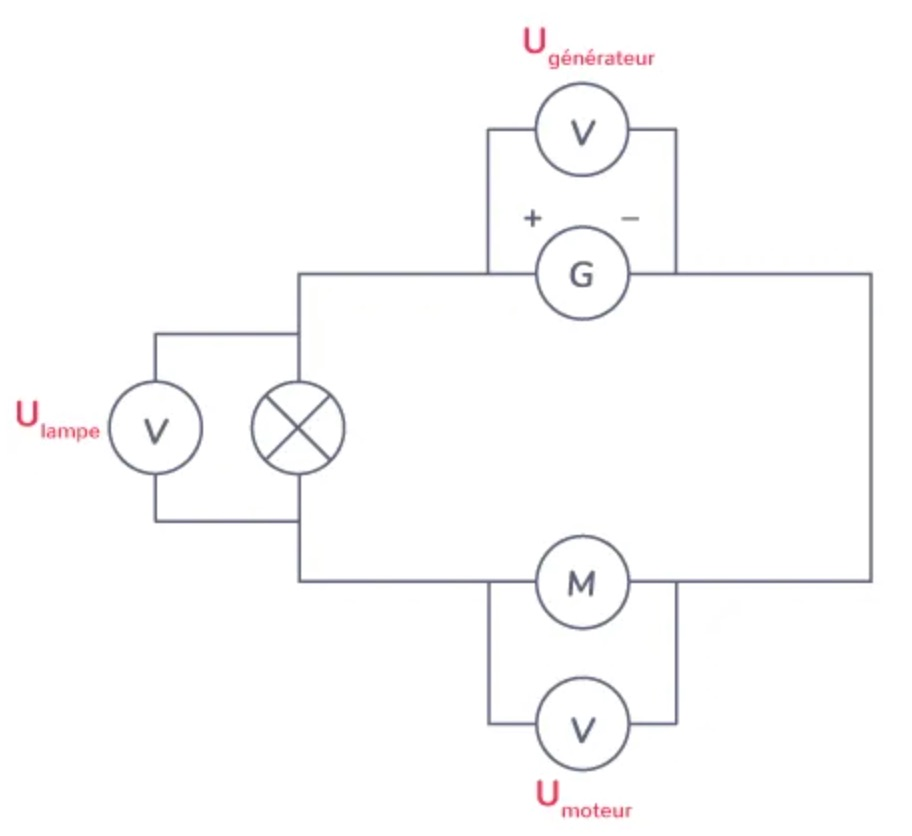
\includegraphics[width=0.5\linewidth]{tension_circuit_2.jpg}
        \captionof{figure}{Circuit électrique 4}
        \end{minipage}}{3}{\(U_\text{générateur} = U_\text{lampe} = U_\text{moteur}\). Loi d'additivité de la tension électrique. Dans un circuit en série, les récepteurs se partagent la tension du générateur. La somme des tensions des dipôles est égale à la tension du générateur.}
    \subsection{Les résistances électriques}
    \item \question{Quelle est la formule de la loi d'Ohm ? Que représentent chaque variables de l'équation, et quelles sont leurs unités ?}{3}{La formule de la loi d'Ohm est \(U = R \times I\), où :
    \begin{itemize}
        \item \(U\) représente la tension électrique, exprimée en volts (V).
        \item \(R\) représente la résistance électrique, exprimée en ohms (\(\Omega\)).
        \item \(I\) représente l'intensité du courant électrique, exprimée en ampères (A).
    \end{itemize}
}
\end{enumerate}

\section{Des signaux pour observer et communiquer}
\subsection{La propagation de la lumière}
\begin{enumerate}
    \item \question{Il existe 2 types de lumière : la lumière visible, et la lumière invisible. Citer 2 exemples de lumières invisibles}{1}{Les rayons infrarouges, ultraviolets, les ondes radios, les rayons gamma, les micro-ondes sont des lumières invisibles (non perceptibles par l'oeil humain)}
    \item \question{Quelle est la vitesse de la lumière dans le vide, en  \unit{\km\per\s} ?}{1}{La vitesse de la lumière dans le vide est de \(\approx 299\,792\,\unit{\km\per\s}\)}
\end{enumerate}

\subsection{La propagation du son}
\begin{enumerate}
    \item \question{A pression et température standard, à quelle vitesse le son se propage-t-il dans le vide ? Et dans l'air (en \si{\m\per\s}) ?}{2}{Dans le vide, le son ne se propage pas. Dans l'air, à pression et température standards, la vitesse du son est d'environ \(343\,\si{\m\per\s}\).}
    \item \question{Quel est le processus expérimental utilisant le son qui permet de mesure la distance entre une source et un obstacle ?}{4}{Le processus expérimental est appelé écholocation ou sonar. Ce procédé consiste à émettre une onde sonore en direction d'un obstacle et à mesurer le temps \(t\) que met l'onde à revenir après avoir été réfléchie. 

    La distance \(d\) entre la source et l'obstacle est alors calculée en utilisant la formule :
    \[
    d = \frac{v \times t}{2}
    \]
    où \(v\) est la vitesse de propagation du son dans le milieu (en \unit{\m\per\s}) et \(t\) est le temps total de l'aller-retour du signal (en \unit{\s}). Le facteur \(\frac{1}{2}\) est utilisé parce que le temps mesuré correspond à un aller-retour, donc la distance parcourue par le son est deux fois la distance entre la source et l'obstacle.}
\end{enumerate}

\end{document}
